\chapter{Historical Context}
Linear A and Linear B were writing systems used during the Bronze Age, primarily on the island of Crete, with some discoveries also made on the Greek mainland.

\section{Historical Introduction}
Around 2000 B.C., the already established Minoan civilization on the island of Crete began constructing large, complex architectural buildings commonly referred to as "palaces."
These edifices served not only as administrative and economic centers, but also played important religious and ceremonial roles within Minoan society.

The founders of these palatial complexes were undoubtedly powerful landowners.
Minoan society was highly organized and capable of mobilizing substantial manpower for the execution of major construction projects, such as the leveling of the hilltops at Knossos and Phaistos, and the erection of monumental palaces on these prepared sites. \cite{alexiou-ch2}

Hence, this highly structured society began to feel the need for a form of administrative writing in order to record transactions, compile inventories, and manage other aspects of economic and bureaucratic activity.

The first form of writing developed by this society was a type of logographic script known as Minoan Hieroglyphics, or Cretan Hieroglyphics, attested between 2100 and 1700 B.C..
The earliest and most archaic script was composed entirely of logographic symbols, which superficially resembled Egyptian hieroglyphs.
It was later abandoned in favor of a linear script known as Linear A, employed between 1800 and 1450 B.C..
The two systems initially coexisted for over a century, but in the following years, Linear A gradually replaced the former and became the sole writing system in use. \cite{salg-ch1}

Notably, the latest attestations of Cretan Hieroglyphs date to around 1700 B.C., when a catastrophe struck the island of Crete.
In fact, all the palaces in the island’s three main centers, Knossos, Phaistos, and Malia were destroyed.
However, this event did not lead to a cultural shift, as the palaces were promptly rebuilt.
This event also determined the passage from the Proto-palatial to the Neo-Palatial phase in Minoan history. \cite{alexiou-ch3}

This second phase of palace construction is the one that has survived to the present day, particularly at sites such as Knossos, Phaistos, Malia, and Zakros.

In 1450 B.C., a major catastrophe struck, probably caused by the eruption of the Thera volcano.
It triggered a series of devastating earthquakes and a powerful tidal wave that swept the north coast of Crete.
As a result, the main centers of Minoan civilization, Phaistos, Aghia Triadha, Malia, the mansions of Tylissos and Ammisos, as well as the eastern cities of Gournia and Zakros, were all reduced to ruins.
The city of Knossos also suffered significant damage, often accompanied by widespread fires. \cite{alexiou-ch4}

In 1400 B.C., Crete began losing its central cultural role, and the focus shifted to mainland Greece, particularly the Peloponnese.
The palace of Knossos got destroyed, while major fortified citadels (fortresses) were built in places like Mycenae and Tiryns. \cite{alexiou-ch5}

During this period, a new linear writing system emerged.
Although the employed script was very similar in form to Linear A, it was adapted to encode a different language: an archaic form of Ancient Greek.
Its name is Linear B, and it was used from 1400 to around 1100 B.C. on the island of Crete and the Greek mainland.
The Mycenaean civilization, which flourished during this period, is characterized by its extensive use of Linear B for administrative purposes, particularly in the context of palace economies.
However, the destruction in Crete should not be interpreted as a Mycenaean military takeover, but rather as a transformative phase of socio-political and cultural adaptation.


\begin{table}[h!]
\centering
\caption{Chronological framework of LA and LB \cite{salg-ch1}}

\begingroup
\renewcommand{\arraystretch}{0.9}
\resizebox{\textwidth}{!}{%
\begin{tabular}{|c|c|c|c|c|c|c|}
\hline
\multicolumn{1}{|c|}{\textbf{Chronology}} & \multicolumn{3}{c|}{\textbf{Crete}} & \multicolumn{3}{c|}{\textbf{Mainland}} \\
\hline
\textbf{High Dating} & \textbf{Pottery Phase} & \textbf{Cultural Phase} & \textbf{Scripts} & \textbf{Pottery Phase} & \textbf{Cultural Phase} & \textbf{Scripts} \\
\hline
1900--1800 & MM II      & \multirow{2}{*}{Proto-Palatial} & CH; LA & MH III   & \multirow{2}{*}{--}               &  -- \\
1800--1700 & MM III     &                                & CH; LA & MH III   &                                 &  -- \\
\hline
1700--1600 & LM IA      & \multirow{2}{*}{Neo-Palatial}   & LA     & LH I     & \multirow{3}{*}{Early Mycenaean} & LA \\
1600--1450 & LM IB      &                                 & LA     & LH IIA   &                                 & ? \\
\cline{1-4}
1450--1400 & LM II      & \multirow{2}{*}{Final-Palatial} & LA?    & LH IIB   &                                 & ? \\
\cline{5-7}
1400--1375 & LM IIIA1   &                                 & LB     & LH IIIA1 & \multirow{4}{*}{Late Mycenaean}  & LB \\
\cline{1-4}
1375--1300 & LM IIIA2   & \multirow{3}{*}{Post-Palatial}  & LB     & LH IIIA2 &                                 & LB \\
 % separate lines for Crete and Mainland
1300--1200 & LM IIIB    &                                 & LB     & LH IIIB  &                                 & LB \\
% separate lines for Crete and Mainland
1200--1050 & LM IIIC    &                                 & --     & LH IIIC  &                                 & LB \\
\hline
\end{tabular}
}
\endgroup
\end{table}


\section{The main sites}
The main sites where Linear A documents have been found are located on the island of Crete. These include Knossos, Phaistos, Aghia Triada, Zakros, Khania, Tylissos, and Malia.

\begin{figure}[H]
    \centering
    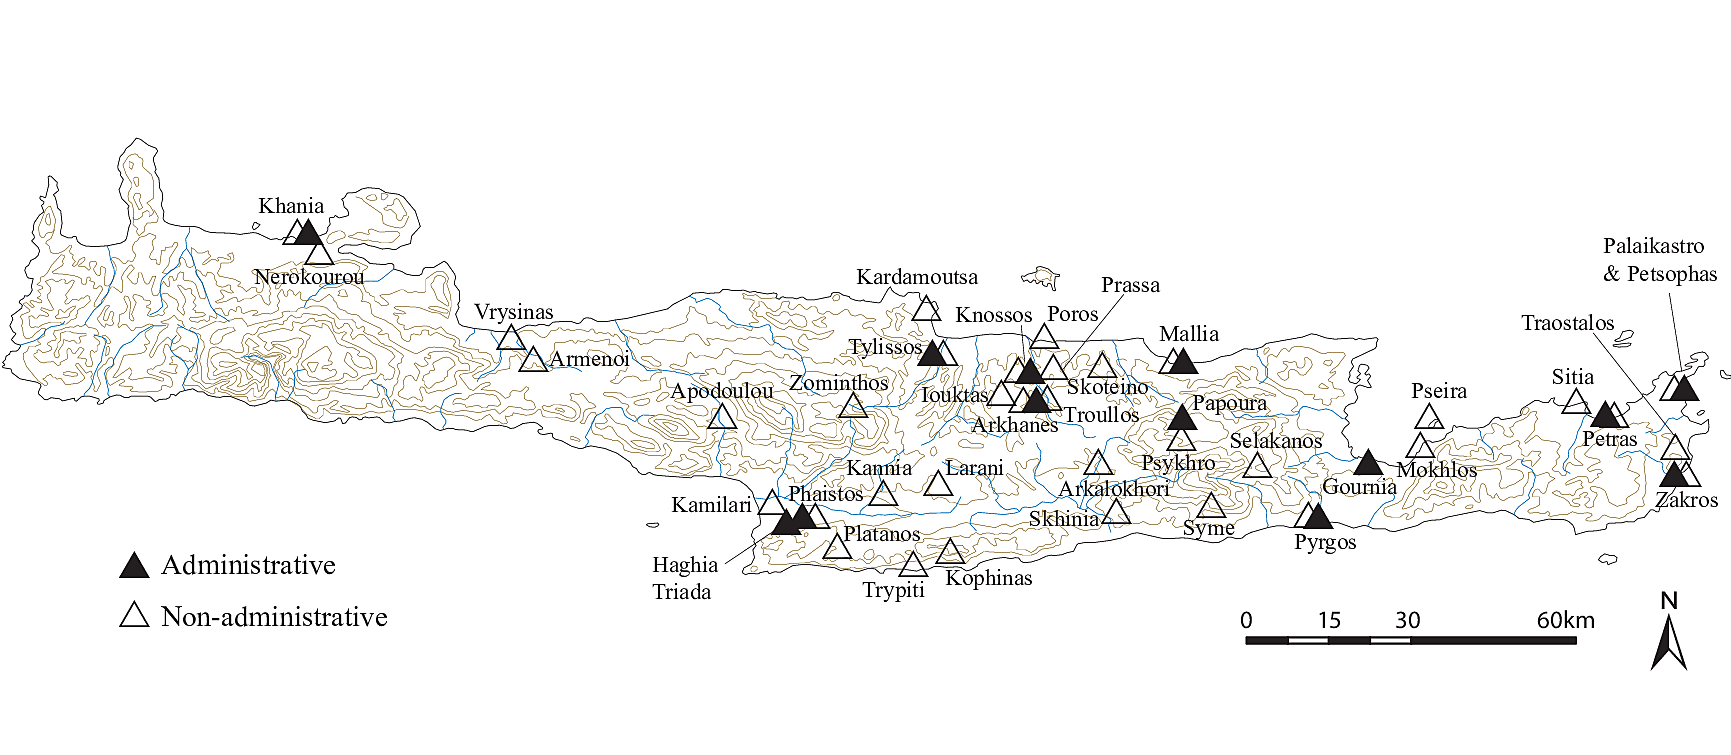
\includegraphics[width=0.8\textwidth]{Images/crete_LA.png} % Adjust width and filename
    \caption{Sites of Linear A fragments in Crete. \protect\footnotemark}
    \label{fig:crete_LA}
\end{figure}
\footnotetext{Figure \ref{fig:crete_LA} prepared by Yannis Galanakis and Ester Salgarella.}

Linear A was more widespread, covering completely Crete and the Aegean Islands and reaching the Greek mainland.
The main attestations of Linear A on the Greek mainland are very limited and generally considered sporadic and isolated. 
At Mycenae, a few Linear A inscriptions have been found, likely as a result of commercial or cultural exchanges with Crete. 
Similarly, some fragmentary finds have been uncovered at Tiryns, probably also related to trade or contacts with Minoan Crete.

\begin{figure}[H]
    \centering
    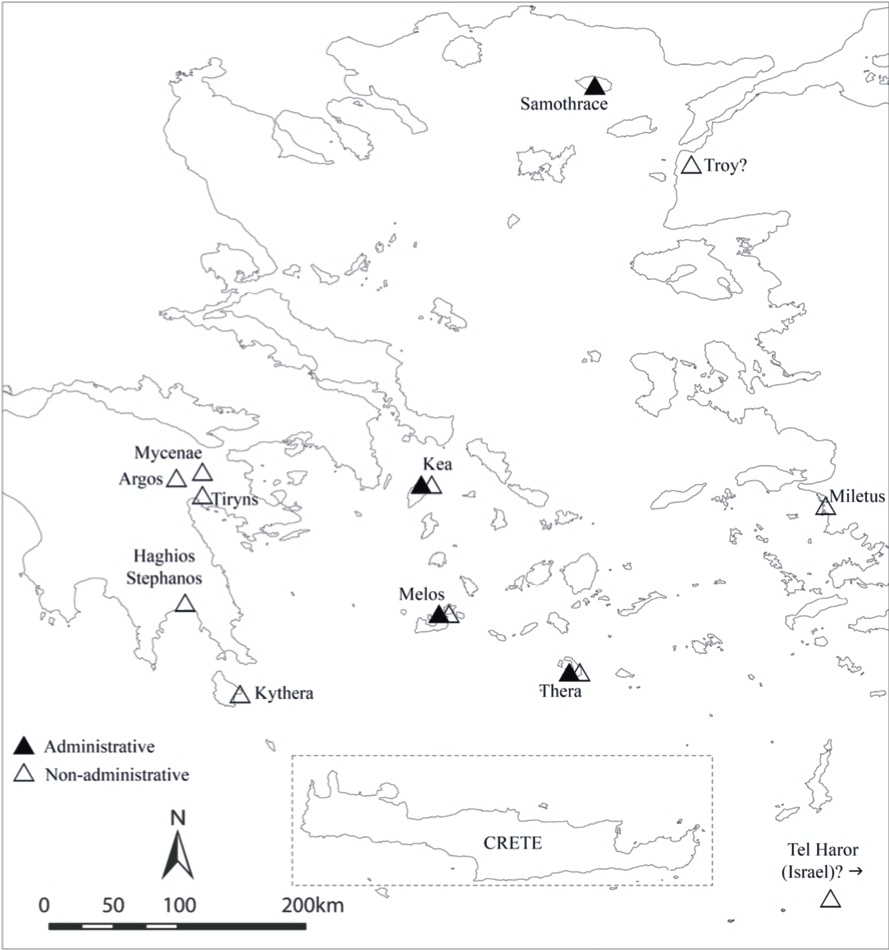
\includegraphics[width=0.8\textwidth]{Images/mainland_LA.jpg} % Adjust width and filename
    \caption{Sites of Linear A fragments in the Greek mainland. \protect\footnotemark}
    \label{fig:mainland_LA}
\end{figure}
\footnotetext{Figure \ref{fig:mainland_LA} prepared by Yannis Galanakis and Ester Salgarella.}

In contrast, Linear B is extensively attested on the Greek mainland, particularly in the Peloponnese, reflecting its administrative function during the Mycenaean period.
Major sites where Linear B documents have been found include Mycenae, Tiryns, Pylos, Thebes, and Athens.
Additionally, significant findings of Linear B tablets have been made in Crete, especially at Knossos and Khania.

The corpora of the two writing systems are relatively small, with Linear A consisting of approximately 1,400 documents, while Linear B comprises around 6,000 documents.
Another notable difference is that Linear A was more widely used for non-administrative purposes, particularly in religious contexts, whereas the number of non-administrative Linear B documents is considerably more limited. \cite{salg-ch1}


\begin{figure}[H]
    \centering
    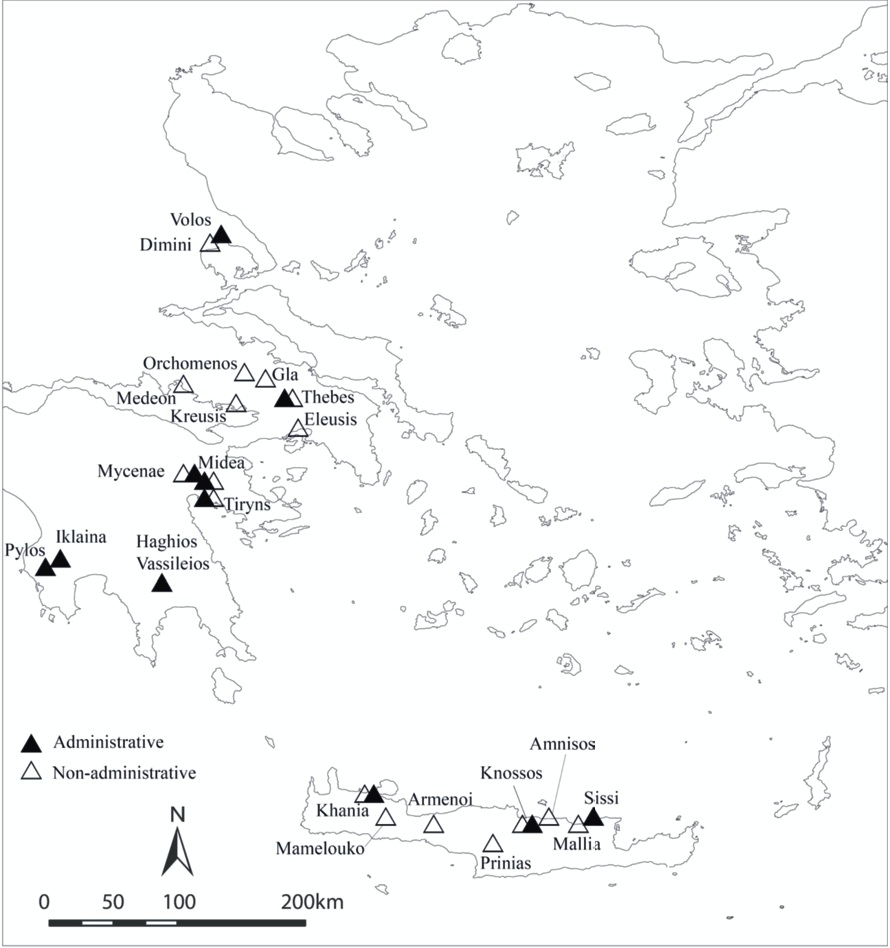
\includegraphics[width=0.8\textwidth]{Images/mainland_LB.jpg} % Adjust width and filename
    \caption{Sites of Linear B fragments in Crete and the Greek mainland. \protect\footnotemark}
    \label{fig:mainland_LB}
\end{figure}
\footnotetext{Figure \ref{fig:mainland_LB} prepared by Yannis Galanakis and Ester Salgarella.}


\section{Linguistic features}
The two writing systems are characterized by similar linguistic features, reflecting the connection between Linear A and Linear B and the derivation of the latter from the former.

The main similarity between the two scripts lies in their syllabic structure, which constitutes a defining feature of both writing systems.
Both Linear A and Linear B are syllabic scripts, meaning that each symbol represents a syllable, rather than an individual letter or a full word.
In addition to syllabic signs, both systems incorporate a set of logograms—symbols representing entire words or concepts.
This logographic component is particularly prominent in Linear A, where a significant number of signs are used to denote specific objects, actions, or concepts, often associated with administrative and religious contexts.
By contrast, Linear B employs a more restricted set of logograms, reflecting its primary function in administrative record-keeping.

Furthermore, a large portion of the Linear A syllabary is shared with Linear B, with approximately 72\% of the Linear A signs being identical to those used in Linear B.
This overlap also illustrates a continuity in symbol creation and in the assignment of phonetic values between the two systems.


\begin{figure}[H]
    \centering
    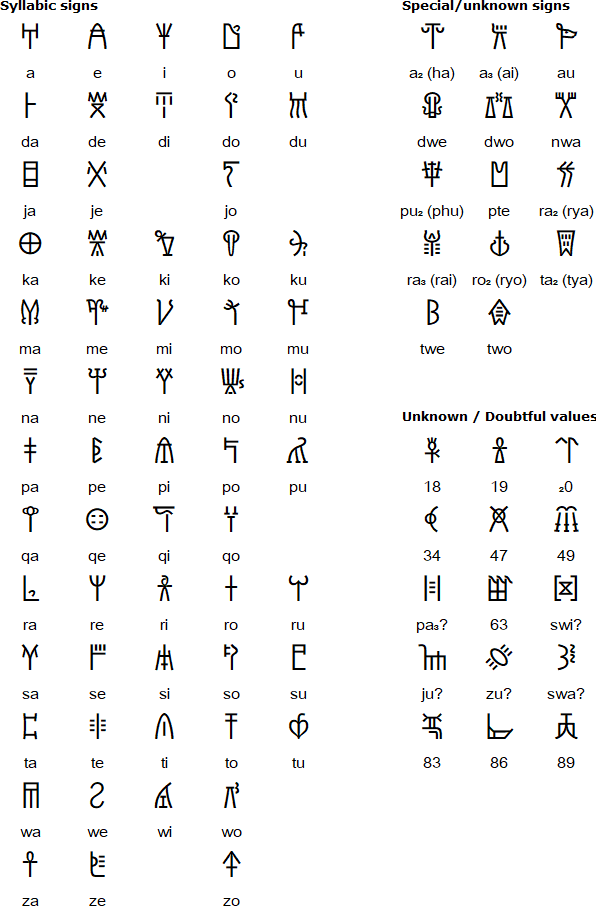
\includegraphics[width=0.8\textwidth]{Images/syll_LB.png} % Adjust width and filename
    \caption{All Linear B syllabograms with the associated phonetic values.}
    \label{fig:syll_LB}
\end{figure}

As can be observed, signs referring to the same vowel exhibit recurring patterns, a characteristic feature of syllabic scripts that is also evident in Linear A.
One of the most debated assumptions regarding the relationship between Linear A and Linear B is the principle of omomorphy and omophony.
This principle posits that signs which are visually similar (omomorphy) in both scripts also share the same phonetic value (omophony), representing the same syllable.
This observation has led to the widely accepted conclusion that Linear A encodes a language fundamentally different from Linear B, the latter being used to represent an archaic form of Ancient Greek.
Consequently, although scholars are able to phonetically transcribe Linear A inscriptions, the meaning of the language remains unknown, as it has not been successfully deciphered.

